% vim: spell spelllang=es:
\documentclass[12pt, oneside]{article}
\usepackage[a4paper, left=2.5cm, right=2.5cm, top=2.5cm, bottom=2.5cm]{geometry}

\usepackage[utf8]{inputenc} % Use unicode
\usepackage[T1]{fontenc}
\usepackage[spanish]{babel} % Names in spanish

%% Bibliography:
%\usepackage{comment}
%\usepackage[
    %backend=biber,
    %style=numeric,
%]{biblatex}
%\DeclareNameAlias{default}{last-first}

%\usepackage{csquotes}       % For bibliography quotations
%\DeclareQuoteAlias{spanish}{catalan}

%\addbibresource{biblio.bib}
%% see:
%% https://www.sharelatex.com/learn/Bibliography_management_in_LaTeX#The_bibliography_file

%\usepackage{datetime} % Customize date
%% \monthyeardate\today gives the date without the day
%\newdateformat{monthyeardate}{%
    %\monthname[\THEMONTH], \THEYEAR}

% For cross references
\usepackage[colorlinks = true]{hyperref}
\usepackage[catalan]{varioref}
%\usepackage{cleveref}
%hyperref configuration so that it doesn't contrast so much colorlinks,
\hypersetup{
   linkcolor={black},
   citecolor={black},
   %linkcolor={red!50!black},
   %citecolor={blue!50!black},
   urlcolor={blue!80!black}
}

\usepackage{mathtools}  % amsmath + more
\usepackage{amsthm}     % Theorem enviroment
\usepackage{amssymb}    % More symbols
\usepackage{amstext}    % Text inside mathenv

\usepackage{relsize}    % Bigger math with mathlarger{___}
\usepackage{nicefrac}   % nice fractions in one line

\usepackage[export]{adjustbox}  % Adjust table size
\usepackage{float}              % Force tables and images position (H and H!)
\usepackage{wrapfig}            % Wrap images like in HTML

\usepackage{tabularx, colortbl, booktabs}    % Better tables
\usepackage{longtable}                      % Multiple page table

% Split cell in lines and more formating options inside table
\usepackage{array, multirow, multicol, makecell}

%\usepackage{subcaption}                     % Subfigures
%\usepackage[framemethod=tikz]{mdframed}     % Custom frames

%\usepackage[bottom]{footmisc} % Footnotes at bottom of page

%\usepackage[alsoload=hep]{siunitx}          % SI units and uncertainties
%\sisetup{locale = FR}                       % Commas and so on for spanish
%\sisetup{separate-uncertainty=true}
%\sisetup{
  %per-mode=fraction,
  %fraction-function=\nicefrac
%}

%\usepackage{tikz}
%%\usetikzlibrary{arrows}
%%\usetikzlibrary{scopes}
%\usetikzlibrary{babel}

%\usepackage{listings}       % For code blocks

%% Custom code highlight
%\definecolor{codegreen}{rgb}{0,0.6,0}
%\definecolor{codegray}{rgb}{0.5,0.5,0.5}
%\definecolor{codepurple}{rgb}{0.58,0,0.82}
%\definecolor{backcolour}{rgb}{0.95,0.95,0.92}
%\definecolor{lightblue}{RGB}{135,206,250}

%\lstdefinestyle{mystyle}{ backgroundcolor=\color{backcolour},
    %commentstyle=\color{codegreen}, keywordstyle=\color{blue},
    %numberstyle=\tiny\color{codegray}, stringstyle=\color{red},
    %identifierstyle=\color{black}, basicstyle=\footnotesize,
    %%breakatwhitespace=false,
    %breaklines=true,
    %%captionpos=b,                    keepspaces=true,
    %numbers=left,                    numbersep=5pt,
    %showspaces=false,
    %%showstringspaces=false, showtabs=false,
    %tabsize=4
%}
%\lstset{style=mystyle}

\newcommand{\whitepage}{
    \clearpage\thispagestyle{empty}\addtocounter{page}{-1} \newpage \clearpage
}

% Add command before appendix session for page numbering: A-1
%\newcommand{\appendixpagenumbering}{
    %\break
    %\pagenumbering{arabic}
    %\renewcommand{\thepage}{\thesection-\arabic{page}}
%}

%% Custom Math operators (functions not in italic in math mode):
%\DeclareMathOperator{\arcsec}{arcsec}
%\DeclareMathOperator{\arccot}{arccot}
%\DeclareMathOperator{\arccsc}{arccsc}
%\DeclareMathOperator{\cis}{cis}


\title{IA Búsqueda local}
\author{%
    Aleix Boné\\
    Alex Herrero\\
    Moisés Balcells
}
\date{%
Marzo 2020
}

% MARIA TERESA ABAD: <mabad@cs.upc.edu>

\begin{document} 

\thispagestyle{empty}
\clearpage
\setcounter{page}{-1}

\begin{titlepage}
{
    \centering
    \null
    \vfill
    {\Large Inteligencia Artificial\par}
    \vspace{2em}
    {\Huge \bfseries 
    Práctica de búsqueda local
    \par}
    \vspace{2em}
    {\large \scshape 
    Marzo 2020
    \par}
    \vfill
\begin{center}
    
\end{center}
    \vspace{3cm}

    \vfill
    {\raggedleft \large
Aleix Boné Ribó\\
Alex Herrero Pons\\
    Moisés Balcells
        \par}
}
\end{titlepage}

\pagebreak

\thispagestyle{empty}
\clearpage
\setcounter{page}{0}

\tableofcontents

\pagebreak


% La documentación deberá incluir:
% La descripción/justificación de la implementación del estado.
% La descripción/justificación de los operadores que habéis elegido...
% La descripción/justificación de las estrategias para hallar la solución inicial.
% La descripción/justificación de las funciones heurísticas.
% Para cada experimento:    
% • Condiciones de cada experimento
% • Resultados del experimento
% • Qué esperabais y qué habéis obtenido    
% • Comparaciones
% • Comentarios adicionales que os parezcan adecuados.
% Comparación entre los resultados obtenidos con Hill Climbing y Simulated Annealing (no olvidéis explicar cómo habéis ajustado los parámetros para este último algoritmo).
% Respuestas razonadas a las preguntas del enunciado.

% Descripción del problema detallada



\section{Descripción del problema}

%Primeramente vamos a describir

\subsection{Elementos del problema}

Los elementos del problema que consisten en un conjunto de servidores y usuarios distribuidos de manera geográfica. Cada
uno de estos servidores tiene a su vez un conjunto de ficheros. Cada fichero esta identificado por un identificador
único y varios servidores pueden tener copias de un mismo fichero (replicaciones) pero no necesariamente todos
los servidores tienen todos los ficheros. Cuando un usuario hace una petición (de un fichero)
un servidor central que se encarga de distribuir las peticiones realizadas por los usuarios. Este servidor tiene información
sobre el contenido de cada uno de los servidores e indica al usuario a que
servidor acceder para obtener el fichero que ha pedido. El servidor que gestiona las peticiones sabe también el tiempo
de transmisión de cada uno de los servidores a cada usuario. Al igual que los ficheros, los servidores, los usuarios y
las peticiones que estos realizan se identifican mediante IDs.

\subsection{Notas importantes}

Los ficheros son servidos de manera secuencial y los tiempos que se tarda en servir una petición no pueden superar a los 5000ms ni bajar de los 100ms. Un usuario puede hacer una o múltiples peticiones de distintos ficheros y un fichero puede ser pedido muchas veces por distintos usuarios.

\subsection{OBJETIVO DEL PROBLEMA}

El objetivo del problema es asignar para cada petición realizada el servidor que servirá el archivo al usuario.
Debemos tener en cuenta que se considera una mejor solución aquella que tiene un menor tiempo de transmisión total y aquella que tiene las cargas de los servidores distribuidas de manera equilibrada. Ya que si únicamente tuvieras en cuenta que fuera el menor tiempo de transmisión total posible las cargas de los servidores no serian equilibradas cosa que no nos interesa.

Así pues, una solución del problema es una asignación para cada petición a un servidor. Debido a que queremos encontrar
una solución que minimiza el tiempo de carga de los servidores y equilibre el trabajo de estos se trata de un problema
de optimización.

\subsection{Variables}

% numero de estados: prop to ~ NREQ*USERS*NREP (TODO: comentar esto en algun sitio)

%nrep/nserv <= 0.5

Las variables que afectan al problema y a las que nos referiremos en el resto de la práctica son las siguientes:

\begin{enumerate}
    \item \texttt{USERS}: número de usuarios.
    \item \texttt{NSERV}: número de servidores.
    \item \texttt{REQUESTS}: máximo numero de peticiones por usuario.
    \item \texttt{NREP}: número de replicaciones mínimo de cada fichero.
\end{enumerate}

Tal como hemos dicho en la sección previa, una solución es una asignación de cada petición a un servidor. Considerando
esto y con las variables del problema que hemos definido tenemos un espacio de soluciones de:
\begin{align}
\texttt{REQUESTS*USERS*REPLICACIONES} \\
\texttt{NREP} \leq \texttt{REPLICACIONES} \leq \texttt{NSERV}
\end{align}

El espacio de soluciones es por lo tanto muy grande para valores relativamente pequeños de usuarios, peticiones y
servidores, por lo que una búsqueda exhaustiva no seria eficiente. Dada una solución válida,
podemos explorar soluciones vecinas cambiando uno de los servidores de una de las peticiones. 

\section{Implementación del estado}

Para lograr el estado inicial con el cuál hemos ejecutado los experimentos hicimos distintas versiones del estado inicial hasta que nos quedamos con la que creíamos que era mejor.

\subsection{Primera versión}

La primera versión de la implementación planteada consistía en lo siguiente, la estructura de datos que hicimos era un array en el cual los índices del array representaban los ids de las peticiones y el contenido de este representaba el servidor con el cual iba a ser servida esa petición, es decir para cada petición en el array guardábamos el servidor que iba a responder esa petición. Los pros y contras que encontramos en esta implementación fueron.

\textbf{Pros:}

-Eficiente en memoria debido a los pocos datos que se almacenan en esta.

\textbf{Contras:}

-El cálculo de las heurísticas es muy lento, ya que al únicamente utilizar esa estructura de datos muchos datos son calculados de manera repetida.

\subsection{Segunda versión}
La segunda versión de la implementación que hicimos consistía en mejorar la primera y las mejoras que añadimos eran añadir otro array. En el cual los índices representaban también los ids de las peticiones, y el contenido de las posiciones del array representaba el tiempo que tarda en servirse dicha petición. Aparte de hacer esta mejora añadimos una variable de tipo entero la cual guardábamos el tiempo total que tardaban en servirse las peticiones.

Las diferencias obtenidas en esta implementación respecto a la  anterior en cuanto al cálculo de las heurísticas  y la eficiencia en la memoria utilizada. Son que el cálculo de las funciones heurísticas tardaba mucho menos que en la primera versión, debido a que hora guardamos variables que antes no guardábamos las cuales nos facilitan el cálculo de las funciones heurísticas, en cuanto a la eficiencia en la memoria esta sigue siendo eficiente pero menos que antes.

\subsection{Versión definitiva}
La última versión de la implementación que realizamos se trataba de una mejora sobre la versión anterior y lo que hicimos fue añadir un hashmap de dos enteros, en este lo que guardamos es el servidor y el tiempo que tarda en servir todas las peticiones que han sido enviadas a ese servidor, es decir guarda el id del servidor y el tiempo en el que sirve todas las peticiones que tiene que servir.

Esta versión final, nos proporciona el menor tiempo de ejecución de todas las versiones anteriores, y teniendo en cuenta que mantiene una eficiencia en memoria aceptable, para el tipo de problemas al que nos enfrentamos creemos que es la mejor opción. 


% primero solo guardavamos para cada req el id del server
% desupes guardamos tambien los tiempos de las req
% finalmente guardamos los tiempos de las req i de los servidores

\section{Operadores que hemos elegido}

\section{Estrategias para hallar la solución inicial}%
\label{sec:estrat_sol}

Implementamos dos estrategias para hallar la solución inicial, una muy naïve que cogía el primer servidor
de la lista de servidores que tenia el fichero para cada petición y otra greedy que cogía para cada petición
el servidor que tenía menor tiempo de transmisión al usuario. La naïve tenía muchos problemas, el principal
que al seleccionar siempre el primer servidor de la lista de servidores que tenían el fichero, la carga de
trabajo se distribuía siempre en los mismos servidores para cada fichero.

\section{Funciones heurísticas}

Implementamos dos funciones heuriticas tal y como pedía el enunciado. La primera minimiza el tiempo de transmisión
de los ficheros para el servidor que necesita mas tiempo para transmitir sus peticiones. La segunda minimiza
el tiempo total de transmisión de los ficheros pero con la restricción de que los tiempos de transmisión de los servidores
han de ser lo más similares possibles entre ellos

\subsection{Primera heurística}

Para la primera heurística simplemente debemos computar el tiempo de transmisión de los ficheros de cada servidor y hallar
el máximo. En nuestra primera versión del estado esto suponía recorrer todas las peticiones y calcular para cada una de
ellas el tiempo de transmisión del servidor al usuario y sumar-lo al tiempo de cada servidor. Después recorríamos los tiempos
de los servidores y encontrábamos el máximo. Este método era lineal en el número de peticiones y de servidores y se tenia
que computar para cada rama de cada estado por el que pasábamos, era por lo tanto muy poco eficiente.

Con la versión definitiva del estado al tener un Map con el tiempo de cada servidor nos ahorramos el paso de
recorrer y computar el tiempo de todas las peticiones y solo tenemos que encontrar el máximo entre los servidores, 
esta operación es lineal en el número de servidores y aunque no lo parezca es mucho más eficiente que la primera
implementación ya que el número de servidores es mucho menor al número de peticiones y no tenemos que hacer
llamadas a las funciones de \texttt{DistFS}.

\subsection{Segunda heurística}

La segunda heurística es más compleja ya que se tienen que considerar dos factores: la minimización del tiempo total
de transmisión y el equilibrio de cargas entre servidores.

Nos decidimos por calcular el tiempo total de transmisión y multiplicar-lo por la desviación estándar de los tiempos
de transmisión de cada servidor.

\section{Experimentos}

\subsection{Influencia de los operadores}

\subsection{Influencia de la solución inicial}

Tal como se ha comentado en la sección~\ref{sec:estrat_sol}, implementamos 2 versiones distintas
para generar la solución inicial. Una que cogía el primer servidor de la lista de servidores que daban ficheros
para cada petición y otra que buscaba entre los servidores que tenían el fichero, el que tenía mínimo
tiempo de transmisión para el usuario de la petición.

La primera versión tenía un coste computacional mínimo ya que solo se accedía al primer elemento del
conjunto retornado por \texttt{DistFS.Server.fileLocations(fileID)}. La otra versión tenia que recorrer
todo el conjunto para encontrar el servidor con tiempo de transmisión mínimo, lo que equivale a un coste
lineal en $NREP$ (Número de replicaciones mínima de un fichero).

A pesar de que la segunda versión del generador de estado inicial es mucho más costoso, esta limitado
por $NREP$ que es una constante y no muy grande ($\nicefrac{NREP}{NSERV} <0.5$), por lo que el coste es negligible
y el tener un mejor estado inicial nos permite llegar a un máximo local con menos iteraciones y que
los máximos locales estén más cerca de un máximo local.

Tal como se especifica en el enunciado de la práctica usamos los mismos parámetros que en el experimento
1 y repetimos el experimento 10 veces en el mismo ordenador para minimizar los efectos externos que
pueden afectar a la solución.

Los resultados obtenidos se muestran en la tabla~\ref{tab:ex2}, en ella
podemos apreciar claramente como el segundo generador (GEN 1) no solo es significativamente más rápido
que el de elegir el primer servidor que se encuentra sino que también llega a un máximo local con
una heurística menor y un tiempo total de transmisión también menor.
Dados los resultados de este experimento decidimos usar el segundo generador para el resto ya que es
mejor en todos los ámbitos analizados.

\begin{table}[H]
    \caption{Resultados del experimento 2}%
    \label{tab:ex2}
    \begin{center}
    \begin{tabular}{lrrrrrrrrr}
\toprule
{} & \multicolumn{3}{c}{time} & \multicolumn{3}{c}{Tiempo total de transmisión} & \multicolumn{3}{c}{Heuristica} \\
{} & repeticiones &    media &       std &                repeticiones &      media &  std & repeticiones &    media &  std \\
GEN &              &          &           &                             &            &      &              &          &      \\
\midrule
0   &        100.0 &  2.18558 &  0.292221 &                       100.0 &  1563778.0 &  0.0 &        100.0 &  91063.0 &  0.0 \\
1   &        100.0 &  1.23535 &  0.029933 &                       100.0 &   559269.0 &  0.0 &        100.0 &  11758.0 &  0.0 \\
\bottomrule
\end{tabular}

    \end{center}
\end{table}

\subsection{Parámetros para el simulated annealing}

\subsection{Evolución del tiempo de ejecución para valores crecientes de los parámetros}

En estos experimentos estudiamos la evolución del coste de la búsqueda en función del tamaño del
problema. Para ello consideramos 2 parámetros: el número de usuarios que piden ficheros y el número
de servidores.

El número de peticiones es como máximo el número de usuarios multiplicado por el número máximo de peticiones
por usuario. Dado que el estado es una asignación de petición a servidor, el número de estados posibles
es el número de de peticiones por el número de replicaciones de cada fichero:

\begin{align}\label{eq:estados}
ESTADOS \approx USERS\cdot REQUESTS \cdot REPLICACIONES \\
NREP \leq REPLICACIONES \leq SERVIDORES
\end{align}

Por lo tanto, el número de estados crece proporcionalmente al número de usuarios, pero no se ve afectado por
el número de servidores ya que un fichero solo puede estar 



\subsubsection{Número de usuarios que piden ficheros}

El número de estados del problema es 


\begin{table}[H]
    \caption{Resultados del experimento 4 (Usuarios)}%
    \label{tab:ex4u}
    \begin{center}
    \begin{tabular}{lrrrr}
\toprule
{} & \multicolumn{2}{l}{time} & \multicolumn{2}{l}{ttt} \\
{} &       media &        std &         media &           std \\
USERS &             &            &               &               \\
\midrule
100   &    0.439545 &   0.344075 &  2.427290e+05 &  20624.964233 \\
200   &    1.782818 &   1.617815 &  4.995559e+05 &  32686.364553 \\
300   &    5.045900 &   0.984051 &  7.645313e+05 &  42743.064831 \\
400   &   10.736700 &   4.973768 &  1.034363e+06 &  51392.984967 \\
500   &   12.388000 &   6.507829 &  1.263917e+06 &  44317.265976 \\
600   &   26.544800 &  12.216475 &  1.543647e+06 &  52970.586044 \\
700   &   34.734900 &  16.169194 &  1.785220e+06 &  67767.572073 \\
800   &   57.239900 &  27.415379 &  2.029594e+06 &  50968.783048 \\
900   &   90.870700 &  26.992538 &  2.305947e+06 &  51138.502401 \\
1000  &  117.450800 &  48.050179 &  2.561704e+06 &  97519.850662 \\
\bottomrule
\end{tabular}

    \end{center}
\end{table}

\begin{figure}[H]
    \centering
    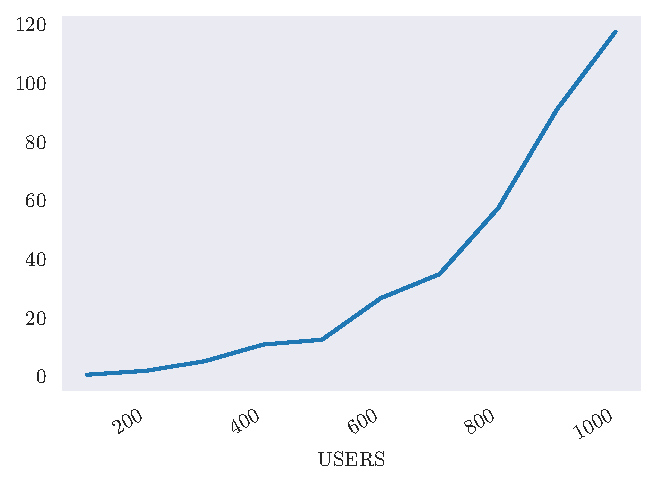
\includegraphics{include/plots/ex4_u_mean_time.pdf}
    \caption{Media Experimento 4 (Usuarios)}%
    \label{fig:ex4u_mean}
\end{figure}

\begin{figure}[H]
    \centering
    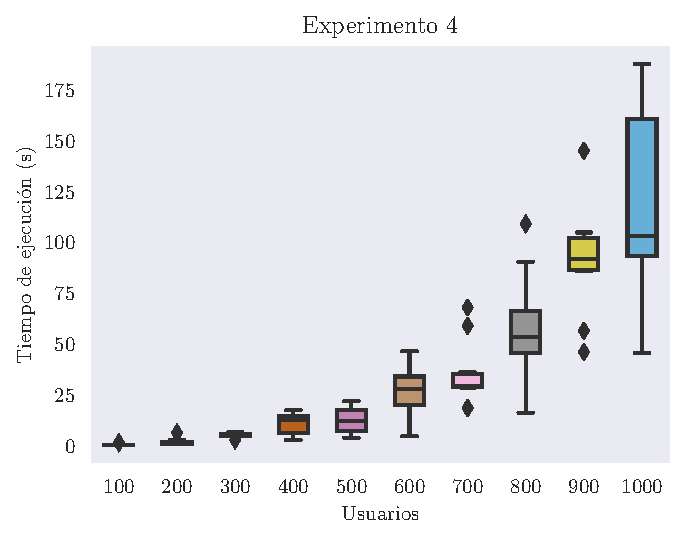
\includegraphics{include/plots/ex4_u_time_bplot.pdf}
    \caption{Experimento 4 (Usuarios)}%
    \label{fig:ex4u}
\end{figure}

\subsubsection{Número de servidores (Manteniendo el número de replicaciones)}

\begin{table}[H]
    \caption{Resultados del experimento 4 (Servidores)}%
    \label{tab:ex4s}
    \begin{center}
    \begin{tabular}{lrrrr}
\toprule
{} & \multicolumn{2}{l}{time} & \multicolumn{2}{l}{ttt} \\
{} &     media &       std &          media &           std \\
NSERV &           &           &                &               \\
\midrule
50    &  4.795824 &  2.562619 &  535961.313725 &  54996.663938 \\
100   &  3.693740 &  1.447718 &  551418.460000 &  36156.093438 \\
150   &  3.343780 &  1.184884 &  545857.920000 &  33942.202363 \\
200   &  2.875980 &  1.162004 &  537334.680000 &  31389.152814 \\
250   &  2.675720 &  0.991247 &  522625.080000 &  36122.916802 \\
300   &  2.281000 &  0.777080 &  519116.800000 &  26411.948652 \\
350   &  2.326820 &  0.899757 &  524597.420000 &  25465.987602 \\
400   &  1.843920 &  0.842095 &  508675.920000 &  29198.579187 \\
450   &  1.869560 &  0.764063 &  510638.680000 &  27791.058100 \\
500   &  1.710100 &  0.580861 &  501650.940000 &  22723.234969 \\
550   &  1.834040 &  0.760056 &  502337.700000 &  21553.327865 \\
600   &  1.497540 &  0.524096 &  506234.960000 &  25396.663981 \\
650   &  1.707580 &  0.588698 &  504194.120000 &  31568.463555 \\
700   &  1.216540 &  0.444400 &  498697.960000 &  21463.111941 \\
750   &  1.368400 &  0.532025 &  498214.900000 &  24553.367374 \\
800   &  1.322060 &  0.544356 &  497294.800000 &  25736.299261 \\
850   &  1.266100 &  0.434882 &  495370.360000 &  26499.868047 \\
900   &  1.236180 &  0.580456 &  502435.000000 &  27949.777197 \\
950   &  1.079920 &  0.439555 &  498911.180000 &  21217.998063 \\
1000  &  1.134480 &  0.433452 &  496641.200000 &  21384.378762 \\
\bottomrule
\end{tabular}

    \end{center}
\end{table}

\begin{figure}[H]
    \centering
    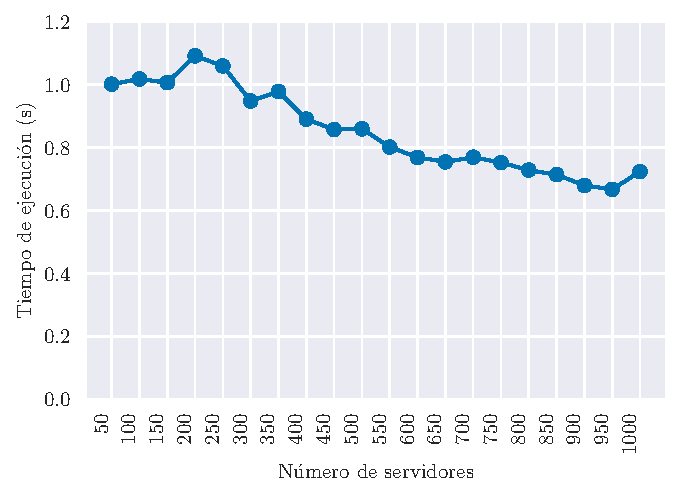
\includegraphics{include/plots/ex4_s_mean_time.pdf}
    \caption{Media Experimento 4 (Servidores)}%
    \label{fig:ex4s_mean}
\end{figure}

\begin{figure}[H]
    \centering
    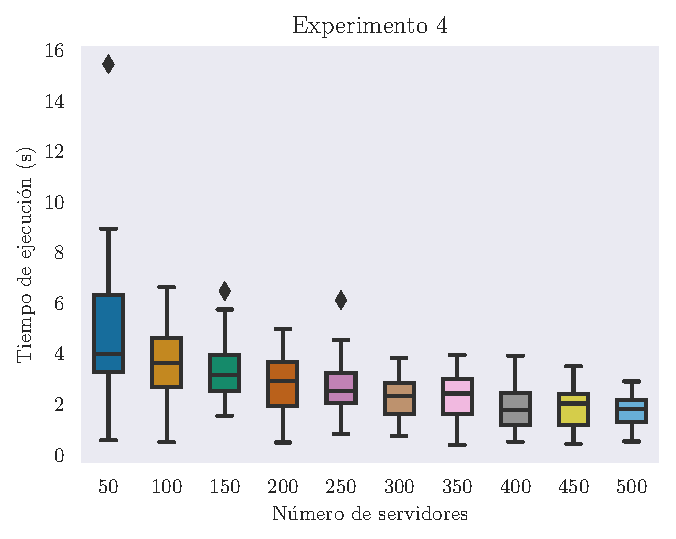
\includegraphics{include/plots/ex4_s_time_bplot_cut.pdf}
    \caption{Experimento 4}%
    \label{fig:ex4s}
\end{figure}

\subsection{Diferencia entre Tiempo total de transmisión y tiempo para hallar la solución (Hill Climbing)}

\subsection{Diferencia entre Tiempo total de transmisión y tiempo para hallar la solución (Simulated Annealing)}

\subsection{Influencia del número de replicaciones de los ficheros}

\begin{table}[H]
    \centering
    \caption{Resultados del experimento 7}%
    \label{tab:ex7}
    \begin{center}
    \begin{tabular}{lrrrr}
\toprule
\multirow{2}{*}{NREP} & \multicolumn{2}{c}{$T_{ej}$} & \multicolumn{2}{c}{TTT} \\
{} &  \makecell{Media} &       \makecell{std}           &      \makecell{Media} & \makecell{std}           \\
\midrule
5    &  1.01077 &  0.332965 &  541711.65 &  34079.558824 \\
10   &  1.43681 &  0.480345 &  342630.67 &  20683.481933 \\
15   &  1.96248 &  0.807076 &  260552.10 &  19601.194839 \\
20   &  2.16906 &  0.928984 &  215671.28 &  16023.596047 \\
25   &  2.62371 &  1.245368 &  191069.57 &  14962.044912 \\
\bottomrule
\end{tabular}

    \end{center}
\end{table}

\begin{figure}[H]
    \centering
    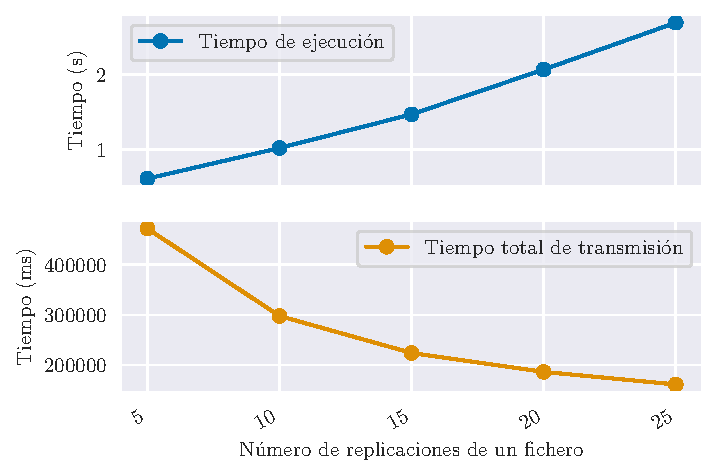
\includegraphics{include/plots/ex7_means.pdf}
    \caption{Medias Experimento 7}%
    \label{fig:ex7means}
\end{figure}

\begin{figure}[H]
    \centering
    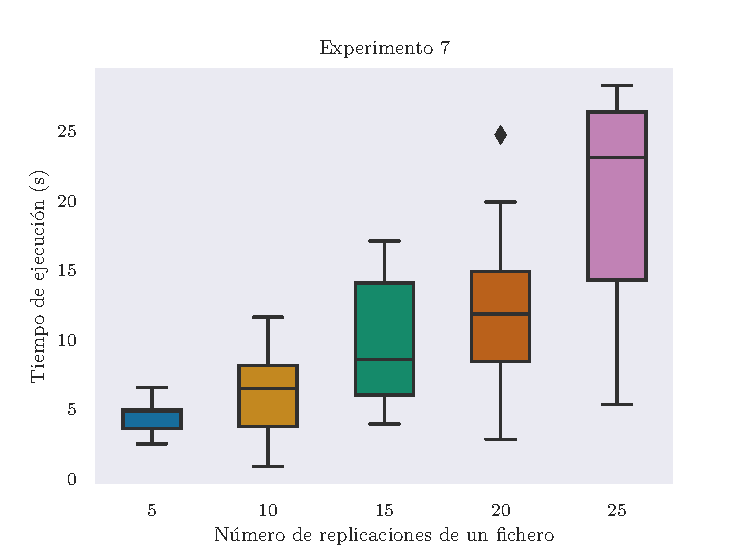
\includegraphics{include/plots/ex7_time_bplot.pdf}
    \caption{Experimento 7}%
    \label{fig:ex7time}
\end{figure}

\begin{figure}[H]
    \centering
    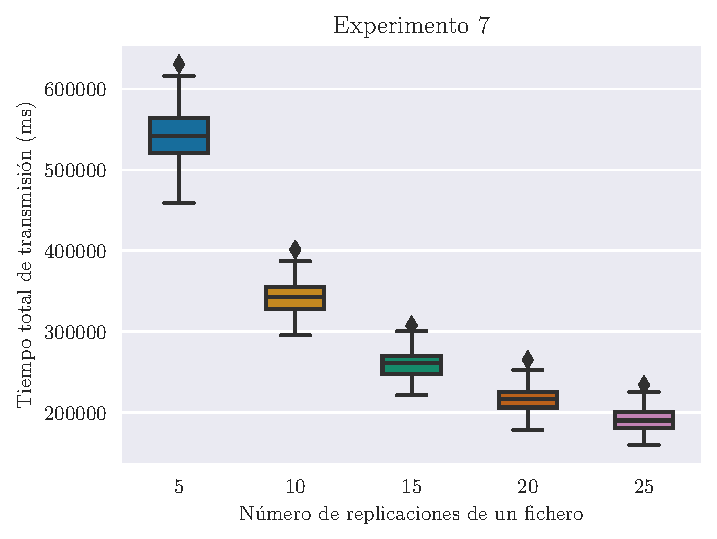
\includegraphics{include/plots/ex7_ttt_bplot.pdf}
    \caption{Experimento 7}%
    \label{fig:ex7ttt}
\end{figure}

\subsection{Conclusión de los experimentos}
    
    
    
\end{document}